\section{Methodology}
\label{sec:methodology}

\subsection{Problem Definition}
\label{sec:problem_definition}

We formulate drug-target interaction (DTI) prediction as a supervised binary
classification problem. Given a drug molecule $D$, a target protein $T$, and a
label $y\in\{0,1\}$ indicating whether the pair interacts, the model learns a
scoring function $f_{\theta}$ that estimates the interaction probability:
\begin{equation}
  s = f_{\theta}(D,T), \qquad
  p = \sigma(s)
  = p_{\theta}(y=1\mid D,T),
  \qquad
  \hat{y} = \mathbf{1}[p\!\ge\!\tau],
  \label{eq:dti_prediction}
\end{equation}
where $s$ is the prediction logit, $\sigma(\cdot)$ is the sigmoid function,
$p\in[0,1]$ is the predicted binding probability, $\tau$ is a
validation-selected decision threshold, $\hat{y}\in\{0,1\}$ is the predicted
binary label, and $\theta$ denotes all trainable parameters. For a mini-batch
$\mathcal{B}=\{(D_i,T_i,y_i)\}_{i=1}^{B}$, the learning objective is to assign
larger logits to interacting pairs and smaller logits to non-interacting pairs.

Each drug is described by three complementary views. The first view is a
SMILES-level molecular language representation extracted from ChemBERTa
\citep{chithrananda2020chemberta}. The second view is a two-dimensional
molecular graph, which preserves atom-level topology and chemical bonds as in
graph-based DTI models \citep{nguyen2021graphdta}. The third view is a set of
three-dimensional conformers encoded with an equivariant geometric network
\citep{satorras2021egnn}. Each target protein is represented by residue-level
ProtBERT features from the ProtTrans family \citep{elnaggar2021prottrans}. The
model must encode each modality, align drug geometry with the paired target,
and perform explicit drug-protein matching.

Throughout this section, $d=128$ denotes the shared hidden dimension. The drug
graph contains at most $N_g=290$ atom tokens, each conformer contains
$N_c=64$ resampled atom tokens, and the main model uses $K=8$ conformers. The
drug token length after topology-geometry concatenation is
$L_d=N_g+N_c=354$. The protein sequence length is denoted by $L_p$, with a
binary mask $\mathbf{m}\in\{0,1\}^{L_p}$ used to identify valid residues.

\subsection{Drug Data Preprocessing}
\label{sec:drug_data_preprocessing}

The preprocessing stage converts each SMILES string into three complementary drug views before neural
encoding. The overview diagram summarizes this conversion in Figure~\ref{fig:drug_preprocess}. The 1D
view captures molecular-language semantics: it is processed by ChemBERTa tokenization, frozen language-
model encoding, and adaptive pooling so that pretrained chemical priors can enter the shared drug-token
interface. The 2D view captures atom-bond topology: it is processed with RDKit/DGLLife graph construction,
canonical atom and bond features, self-loops, and virtual-node padding so that local chemical connectivity is
preserved. The 3D view captures plausible ligand geometry: it is processed through hydrogen addition, ETKDG
conformer generation, optional UFF optimization, energy ranking, fixed-size atom-token pooling, and validity
masking so that the downstream model can choose among multiple target-dependent conformations rather than
relying on a single fixed geometry.

\paragraph{1D semantic preprocessing.}
The 1D module treats the SMILES string as a molecular language sequence. The string is tokenized and encoded
by a frozen ChemBERTa-77M-MTR model \citep{chithrananda2020chemberta}. Special tokens are removed, and the
remaining token hidden states are adaptively pooled to the shared drug-token length and hidden dimension,
giving $\mathbf{X}_{\mathrm{chem}}\in\mathbb{R}^{354\times128}$. This branch provides pretrained chemical
semantics and remains independent of atom-index ordering in the graph and conformer branches.

\paragraph{2D topology preprocessing.}
The 2D module reconstructs the molecular graph from the same SMILES string using RDKit and DGLLife. Canonical
atom and bond featurizers build a DGL molecular bigraph with self-loops, atom descriptors, bond descriptors,
and adjacency structure. Atom features are augmented with a virtual-node indicator and padded with virtual
nodes to $N_g=290$ graph nodes, producing the graph input $\mathcal{G}_D$. This branch preserves local
chemical connectivity and bond-induced neighborhood structure that are not explicit in the pooled ChemBERTa
token matrix.

\paragraph{3D conformer preprocessing.}
The 3D module generates candidate ligand geometries. Hydrogens are first added, then RDKit ETKDGv3 embeds up
to $K$ conformers. When UFF parameters are available, each conformer is optimized and assigned a computed
UFF energy. The candidate conformers are sorted by this energy, adaptively pooled to $N_c=64$ atom tokens,
and stored as atom features $\mathbf{F}_k$, Cartesian coordinates $\mathbf{R}_k$, normalized energy
$\epsilon_k$, and validity indicator $q_k$. Invalid or missing conformer slots are zero-padded and masked.
This module therefore exposes multiple plausible geometries to the later target-aware conformer selector,
rather than committing to a single fixed conformation during preprocessing.

Together, the three modules produce the cached drug-side inputs
$\mathbf{X}_{\mathrm{chem}}$, $\mathcal{G}_D$, and
$\{\mathbf{F}_k,\mathbf{R}_k,\epsilon_k,q_k\}_{k=1}^{K}$ used by the drug encoder.

\begin{figure}[!htbp]
\centering
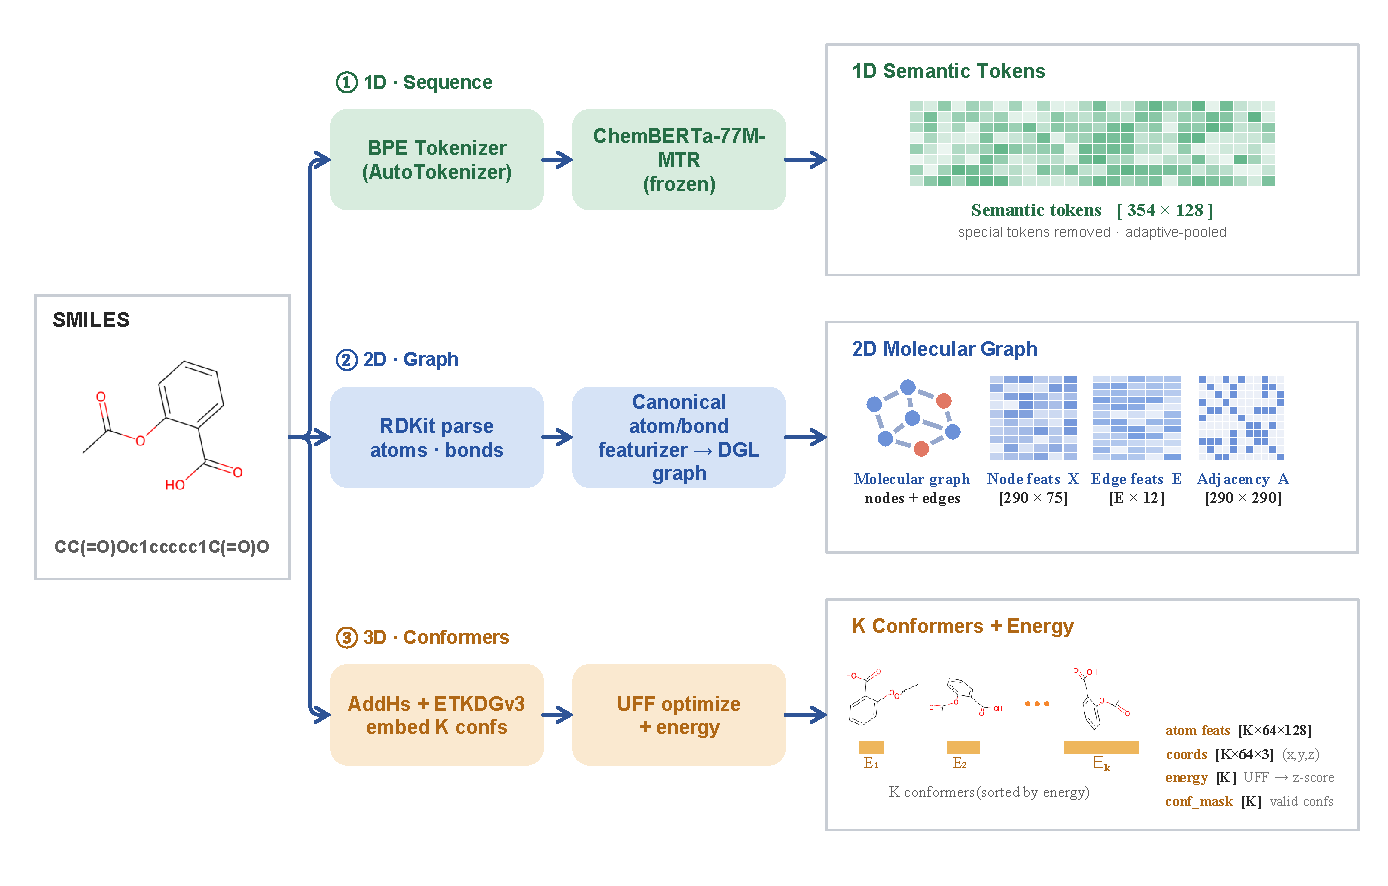
\includegraphics[width=\linewidth]{figures/drug_preprocess.pdf}
\caption{Drug data preprocessing. Starting from a SMILES string, TAMR-DTI
constructs a ChemBERTa semantic-token matrix, an RDKit/DGL molecular graph, and
a set of energy-ranked 3D conformers with atom features, coordinates, energies,
and conformer-validity indicators.}
\label{fig:drug_preprocess}
\end{figure}
\FloatBarrier

\subsection{Proposed Representation Framework}
\label{sec:overall_framework}

The proposed TAMR-DTI representation framework is built on a BiIntention-based DTI backbone
\citep{peng2024bindti,ji2026ldmdti}. It is organized into six modules that are detailed in the following
module descriptions. The drug representation module constructs a fused ligand token sequence from
ChemBERTa semantics, graph topology, and target-aware conformer geometry. The protein representation module
maps ProtBERT residue features into ligand-conditioned protein tokens through FiLM-modulated ACmix blocks.
The aligned representation interface standardizes hidden dimensions, token lengths, context vectors, and
masks before cross-modal comparison. The protein representation refinement and interaction module applies
gated bidirectional Mamba only to the ordered protein token stream and then uses BiIntention for explicit
drug-target matching \citep{gu2022s4,gu2023mamba}. The prediction module converts the resulting interaction
representation into a binding logit, and the training objective optimizes this logit with weighted binary
cross-entropy.

The schematic overview in Figure~\ref{fig:tamr_dti_architecture} and the formal flow in
Eq.~\ref{eq:overall_pipeline} summarize the end-to-end representation path. The drug representation module
receives the ChemBERTa semantic tokens, the molecular graph, the conformer cache, and the initial protein
seed representation. It extracts topology and target-conditioned geometry, then fuses the drug-side streams
into the token sequence $\mathbf{D}$. The fused drug tokens are pooled into the ligand context $\mathbf{x}_D$,
which conditions the protein representation module. A gated bidirectional Mamba residual block refines the
ligand-conditioned protein tokens, BiIntention forms the compact interaction representation, and the
prediction module maps this representation to the interaction probability.

\begin{figure}[!htbp]
\centering
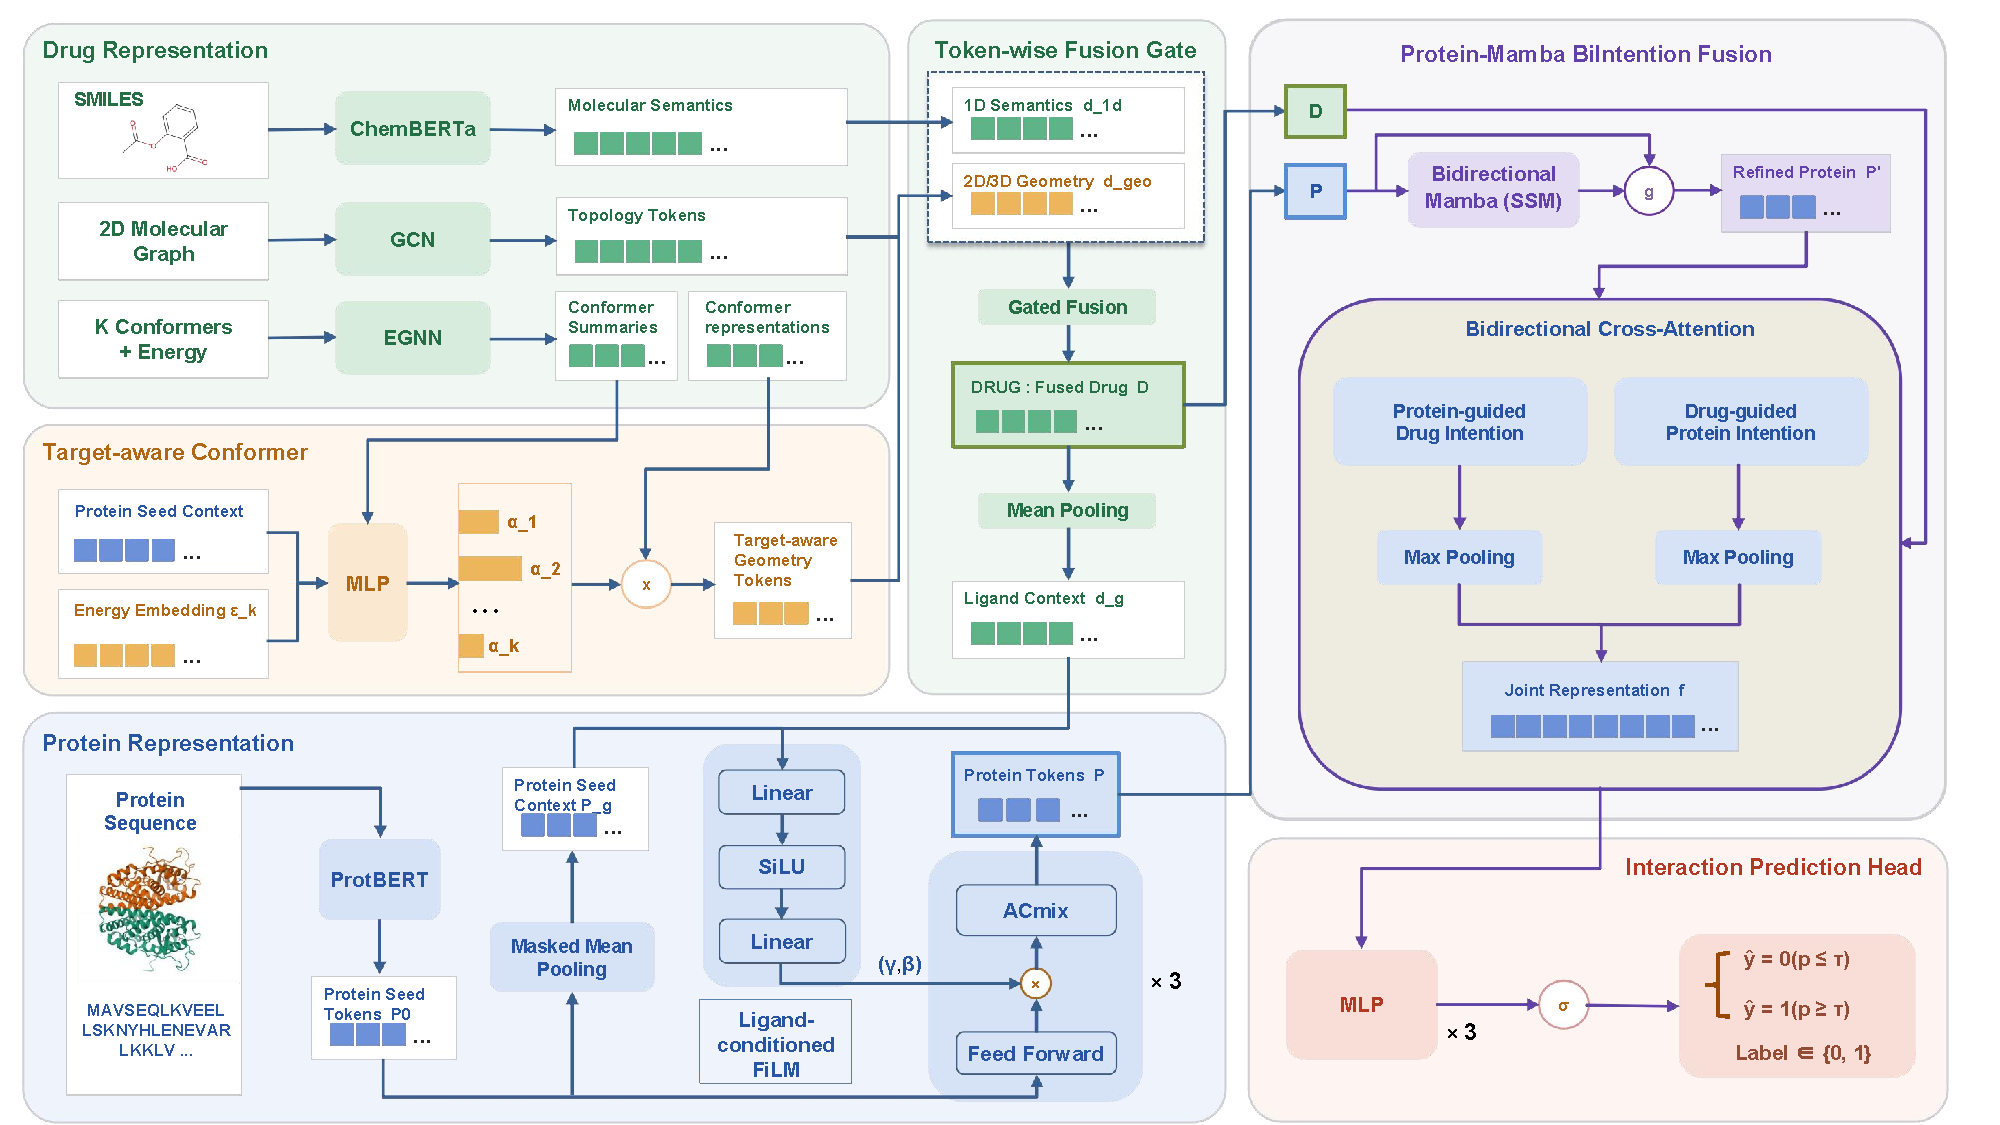
\includegraphics[width=\linewidth]{figures/tamr_dti_architecture.pdf}
\caption{TAMR-DTI representation framework. The figure is a schematic view of the drug representation
streams, ligand-conditioned protein representation module, protein representation refinement block, and
BiIntention interaction representation head. Formal tensor notation is defined in Eq.~\ref{eq:overall_pipeline}
and the surrounding text. Glyphs: $\boldsymbol{\times}$ multiplication, $\odot$ element-wise product,
$\sigma$ sigmoid, and ``$\times 3$'' a block stacked three times.}
\label{fig:tamr_dti_architecture}
\end{figure}

The computation is
\begin{equation}
\begin{aligned}
  \mathbf{D} &=
  \operatorname{DrugEnc}\!\left(
    \mathbf{X}_{\mathrm{chem}},\mathcal{G}_D,
    \{\mathbf{F}_k,\mathbf{R}_k,\epsilon_k,q_k\}_{k=1}^{K},
    \mathbf{P}^{0},\mathbf{m}
  \right), \\
  \mathbf{x}_D &=
  \operatorname{MeanPool}(\mathbf{D}),\\
  \mathbf{P} &= \operatorname{ProtEnc}\!\left(
    \mathbf{P}^{0},\mathbf{m},\mathbf{x}_D
  \right),\\
  \mathbf{P}' &=
  \operatorname{ProtMamba}(\mathbf{P},\mathbf{m}),\\
  \mathbf{f} &= \operatorname{BiIntention}(\mathbf{D},\mathbf{P}'),\\
  s &= \operatorname{MLP}(\mathbf{f}), \qquad
  p=\sigma(s).
\end{aligned}
\label{eq:overall_pipeline}
\end{equation}
Here $\mathbf{X}_{\mathrm{chem}}\in\mathbb{R}^{L_d\times d}$ denotes the ChemBERTa drug
feature sequence, $\mathcal{G}_D$ is the molecular graph,
$(\mathbf{F}_k,\mathbf{R}_k)$ are the atom features and coordinates of conformer
$k$, $\epsilon_k$ is its conformer energy, and $q_k\in\{0,1\}$ marks whether the
conformer is valid. $\mathbf{P}^{0}$ is the projected ProtBERT protein feature,
$\mathbf{D}\in\mathbb{R}^{L_d\times d}$ is the fused drug token sequence,
$\mathbf{P}\in\mathbb{R}^{L_p\times d}$ is the ligand-conditioned protein token
sequence before protein-side Mamba refinement, $\mathbf{P}'$ is the
refined protein token sequence, $\mathbf{x}_D$ is the global ligand context used
for ligand-conditioned protein encoding, and $\mathbf{f}\in\mathbb{R}^{2d}$ is
the fused pair representation. The projected protein sequence first guides
conformer aggregation, and the resulting drug representation then provides
ligand context for protein encoding before final cross-modal matching.

\subsubsection{Drug Representation Module}
\label{sec:drug_representation_module}

The drug representation module integrates molecular language, graph topology,
and target-aware 3D geometry. SMILES features encode chemical semantics learned
from molecular corpora, graph features preserve atom-neighbor connectivity, and
conformer features encode spatial arrangement. TAMR-DTI first represents the
one-dimensional SMILES stream with a frozen molecular language model, computes
topology and geometry tokens from RDKit-derived structures, and then fuses the
three drug views through a learnable gate.

\paragraph{1D semantic representation.}
The 1D branch starts from the SMILES string $s_D$ and treats it as a molecular
language sequence. During preprocessing, $s_D$ is tokenized with the ChemBERTa
tokenizer and encoded by the frozen ChemBERTa-77M-MTR backbone:
\begin{equation}
  \mathbf{U}^{\mathrm{chem}}=\operatorname{ChemBERTa}(s_D)
  \in\mathbb{R}^{L_s\times d_c}.
  \label{eq:chemberta_encoding}
\end{equation}
Here $L_s$ and $d_c$ denote the ChemBERTa sequence length and hidden size
before fixed-size pooling. Special tokens are removed, and the remaining token
hidden states are pooled to the shared drug-token length and hidden dimension:
\begin{equation}
  \mathbf{X}_{\mathrm{chem}}=\operatorname{Pool}_{L_d,d}
  \left(\mathbf{U}^{\mathrm{chem}}_{\neg\mathrm{special}}\right)
  \in\mathbb{R}^{L_d\times d}.
  \label{eq:chemberta_pooling}
\end{equation}
The resulting sequence provides pretrained SMILES semantics. Its positions are
fixed molecular-language slots after pooling, not atom indices, which is why the
later fusion gate is interpreted as a latent-slot fusion rather than a direct
SMILES-token-to-atom alignment.

\paragraph{2D topology representation.}
Let $\mathcal{G}_D=(\mathcal{V},\mathcal{E})$ be the padded molecular graph of
drug $D$, where each atom node has an input feature
$\mathbf{a}_i\in\mathbb{R}^{75}$. The implementation first projects atom
features to the hidden space:
\begin{equation}
  \mathbf{h}^{g,0}_i = \mathbf{W}_g\mathbf{a}_i,
  \qquad
  \mathbf{H}^{g,0}\in\mathbb{R}^{N_g\times d}.
  \label{eq:gcn_projection}
\end{equation}
When graph padding is enabled, the last input channel is used as the virtual
padding marker, and its projection weight is fixed to zero so that padded nodes
do not introduce artificial atom semantics. A multi-layer graph convolutional
network then aggregates local chemical topology:
\begin{equation}
  \mathbf{H}^{g} =
  \operatorname{GCN}(\mathcal{G}_D,\mathbf{H}^{g,0})
  \in\mathbb{R}^{N_g\times d}.
  \label{eq:gcn_output}
\end{equation}
The resulting $\mathbf{H}^{g}$ provides atom-level topology tokens.

\paragraph{3D conformer representation.}
For conformer $k$, let
$\mathbf{F}_k\in\mathbb{R}^{N_c\times d}$ denote atom features and
$\mathbf{R}_k\in\mathbb{R}^{N_c\times 3}$ denote Cartesian coordinates. TAMR-DTI
uses an EGNN layer to update atom features while respecting Euclidean symmetry:
\begin{equation}
  (\mathbf{Z}_k,\mathbf{R}'_k)
  =
  \operatorname{EGNN}(\mathbf{F}_k,\mathbf{R}_k),
  \qquad
  \mathbf{Z}_k\in\mathbb{R}^{N_c\times d}.
  \label{eq:egnn_conformer}
\end{equation}
The conformer-level summary is obtained by average pooling over the fixed
resampled atom tokens:
\begin{equation}
  \mathbf{c}_k =
  \frac{1}{N_c}\sum_{i=1}^{N_c}\mathbf{z}_{k,i}.
  \label{eq:conformer_global}
\end{equation}
This summary is used only to score conformer relevance; the final 3D drug
representation remains atom-resolved.

The conformer slots are kept in the order produced by preprocessing. RDKit
ETKDG is used to generate candidate conformers, UFF optimization is applied when
force-field parameters are available, and the resulting conformers are sorted by
their computed UFF energy before padding or truncation. Therefore, the first slot
corresponds to the lowest computed-energy conformer among the generated
candidates, slots two to four provide lower-energy alternative conformations,
and later slots contain higher-energy generated alternatives. The energy value
is used as an auxiliary conformer-ranking feature rather than as a calibrated
cross-molecule thermodynamic quantity. The conformer-count comparison follows
this order: the $n=1$ setting tests a fixed lowest-computed-energy
geometry, whereas larger $n$ values expose progressively broader geometric
alternatives to the target-aware selector.

\paragraph{Target-aware conformer representation.}
Conformer aggregation depends on the paired protein. The same ligand can expose
different binding-relevant geometric cues for different targets, so a fixed
conformer average may dilute target-specific 3D signal. ProtBERT tokens are
first normalized and projected:
\begin{equation}
  \mathbf{P}^{0} =
\mathbf{W}_p\,\operatorname{LayerNorm}(\mathbf{P}_{\mathrm{ProtBERT}}),
  \qquad
  \mathbf{P}_{\mathrm{ProtBERT}}\in\mathbb{R}^{L_p\times 1024},
  \quad
  \mathbf{P}^{0}\in\mathbb{R}^{L_p\times d}.
  \label{eq:protein_seed_projection}
\end{equation}
The masked protein context vector is then
\begin{equation}
  \mathbf{x}_T =
  \frac{\sum_{j=1}^{L_p}m_j\mathbf{p}^{0}_j}
       {\max(1,\sum_{j=1}^{L_p}m_j)}.
  \label{eq:protein_context}
\end{equation}
For each conformer, its energy $\epsilon_k$ is projected to the hidden space,
$\mathbf{u}_k=\mathbf{W}_{e}\epsilon_k$. The conformer logit combines the
conformer summary, the protein context, and the energy embedding:
\begin{equation}
  a_k =
  \mathbf{w}_{a}^{\top}
  \operatorname{SiLU}
  \left(
    \mathbf{W}_{a}
    [\mathbf{c}_k;\mathbf{x}_T;\mathbf{u}_k]
    +\mathbf{b}_{a}
  \right)
  + b_s.
  \label{eq:conformer_score}
\end{equation}
Invalid conformers are masked by assigning their logits a large negative value.
For samples with at least one valid conformer, the conformer weights are
\begin{equation}
  \alpha_k =
  \frac{\exp(a_k)\,q_k}
       {\sum_{\ell=1}^{K}\exp(a_{\ell})\,q_{\ell}},
  \qquad
  \sum_{k=1}^{K}\alpha_k=1.
  \label{eq:conformer_weight}
\end{equation}
In the rare case that preprocessing yields an empty conformer-validity mask, the
implementation activates the first conformer slot as a fallback before applying
the softmax, preventing a zero denominator in Eq.~\ref{eq:conformer_weight}.
The target-aware atom-level 3D representation and its global context are
\begin{equation}
  \mathbf{Z}^{3D}
  =
  \sum_{k=1}^{K}\alpha_k\mathbf{Z}_k,
  \qquad
  \mathbf{c}^{3D}
  =
  \sum_{k=1}^{K}\alpha_k\mathbf{c}_k.
  \label{eq:target_aware_3d}
\end{equation}
Thus, conformer weights are conditioned on the paired protein rather than fixed
for the ligand alone.

\paragraph{Drug representation fusion.}
The graph topology tokens and target-aware 3D tokens are concatenated:
\begin{equation}
  \mathbf{X}_{\mathrm{str}} =
  [\mathbf{H}^{g};\mathbf{Z}^{3D}]
  \in\mathbb{R}^{(N_g+N_c)\times d}.
  \label{eq:geo_concat}
\end{equation}
By construction, this structural sequence has length
$N_g+N_c=L_d$ and matches the 1D ChemBERTa feature sequence
$\mathbf{X}_{\mathrm{chem}}\in\mathbb{R}^{L_d\times d}$. Therefore, the fusion
gate should be understood as a fixed latent-slot operation over two equal-length
drug representations after preprocessing. The slot index does not imply a
one-to-one chemical alignment between a SMILES token and a graph atom. Both
branches are normalized and combined by a slot-wise, channel-wise gate:
\begin{equation}
\begin{aligned}
  \tilde{\mathbf{X}}_{\mathrm{chem}}
  &= \operatorname{LayerNorm}(\mathbf{X}_{\mathrm{chem}}),\\
  \tilde{\mathbf{X}}_{\mathrm{str}}
  &= \operatorname{LayerNorm}(\mathbf{X}_{\mathrm{str}}),\\
  \mathbf{G}^{D}
  &= \sigma\!\left(
      \mathbf{W}_{f}
      [\tilde{\mathbf{X}}_{\mathrm{chem}};\tilde{\mathbf{X}}_{\mathrm{str}}]
      +\mathbf{b}_{f}
    \right),\\
  \mathbf{D}
  &= \mathbf{G}^{D}\odot\tilde{\mathbf{X}}_{\mathrm{chem}}
   + (1-\mathbf{G}^{D})\odot\tilde{\mathbf{X}}_{\mathrm{str}}.
\end{aligned}
\label{eq:drug_gate}
\end{equation}
The gate bias is initialized to $-2.0$, so the initial value
$\sigma(-2.0)\approx0.119$ assigns a small but nonzero weight to the ChemBERTa
branch and a larger initial weight to the topology-geometry branch. During
training, the gate learns the token-wise balance between pretrained molecular
semantics and structural information. The global ligand context used by the
protein module is
\begin{equation}
  \mathbf{x}_D = \frac{1}{L_d}\sum_{i=1}^{L_d}\mathbf{d}_i.
  \label{eq:drug_context}
\end{equation}

\subsubsection{Protein Representation Module}
\label{sec:protein_representation_module}

The protein representation module maps ProtBERT residue features into ligand-conditioned
protein tokens. ProtBERT provides residue-level sequence priors, and the
Feature-wise Linear Modulation (FiLM) path \citep{perez2018film} lets the paired
ligand modulate these tokens before cross-modal fusion.

The input protein sequence is first mapped from the ProtBERT dimension to the
shared hidden dimension using Eq.~\ref{eq:protein_seed_projection}. This is the
same protein seed sequence used by the drug representation module for target-aware
conformer selection. The projected tokens $\mathbf{P}^{0}$ are then passed through
three ProteinACmix layers. Each layer
combines a feed-forward half-step, ligand-conditioned feature modulation,
relative self-attention, dynamic convolution, and a second feed-forward
half-step. For layer $\ell=1,\ldots,3$, let
$\mathbf{P}^{\ell-1}\in\mathbb{R}^{L_p\times d}$ be the input tokens. The first
feed-forward residual update is
\begin{equation}
  \mathbf{U}^{\ell}
  =
  \frac{1}{2}\operatorname{FFN}^{\ell}_{1}(\mathbf{P}^{\ell-1})
  +
  \frac{1}{2}\mathbf{P}^{\ell-1}.
  \label{eq:protein_ffn_half_1}
\end{equation}
If ligand conditioning is enabled, the global drug context $\mathbf{x}_D$ is
converted into feature-wise scale and shift parameters
$\boldsymbol{\gamma}^{\ell},\boldsymbol{\beta}^{\ell}\in\mathbb{R}^{d}$:
\begin{equation}
\begin{aligned}
  \bigl[\boldsymbol{\gamma}^{\ell},\boldsymbol{\beta}^{\ell}\bigr]
  &= \operatorname{MLP}^{\ell}_{film}(\mathbf{x}_D),\\
  \bar{\boldsymbol{\gamma}}^{\ell}
  &= \rho\tanh(\boldsymbol{\gamma}^{\ell}),\\
  \bar{\boldsymbol{\beta}}^{\ell}
  &= \rho\boldsymbol{\beta}^{\ell},
\end{aligned}
\qquad \rho=0.05.
\label{eq:film_params}
\end{equation}
The protein tokens are then modulated as
\begin{equation}
  \tilde{\mathbf{U}}^{\ell}
  =
  \mathbf{U}^{\ell}\odot
  (1+\bar{\boldsymbol{\gamma}}^{\ell})
  +\bar{\boldsymbol{\beta}}^{\ell}.
  \label{eq:ligand_film}
\end{equation}
where the scale and shift vectors are broadcast over the residue-token axis.
When ligand conditioning is disabled, the implementation uses
$\tilde{\mathbf{U}}^{\ell}=\mathbf{U}^{\ell}$. The fixed scale $\rho$ keeps
ligand modulation small at initialization.

The modulated tokens are further processed by the CNN-Transformer block:
\begin{equation}
\begin{aligned}
  \mathbf{A}^{\ell}
  &=
  \operatorname{MHSA}_{rel}^{\ell}
  (\tilde{\mathbf{U}}^{\ell},\mathbf{m})
  +\tilde{\mathbf{U}}^{\ell},\\
  \mathbf{C}^{\ell}
  &=
  \operatorname{Conv}^{\ell}(\mathbf{A}^{\ell})
  +\mathbf{A}^{\ell},\\
  \mathbf{P}^{\ell}
  &=
  \frac{1}{2}\operatorname{FFN}^{\ell}_{2}(\mathbf{C}^{\ell})
  +
  \frac{1}{2}\mathbf{C}^{\ell}.
\end{aligned}
\label{eq:protein_acmix}
\end{equation}
The relative multi-head self-attention captures long-range residue dependencies
under the protein mask, and the convolutional branch emphasizes local sequence
motifs that may be relevant to interaction prediction. After three layers, the
protein module outputs
\begin{equation}
  \mathbf{P}=\mathbf{P}^{3}
  \in\mathbb{R}^{L_p\times d}.
  \label{eq:protein_output}
\end{equation}

\subsubsection{Aligned Representation Interface}
\label{sec:feature_encoder_module}

The preceding representation modules operate on heterogeneous inputs: cached
ChemBERTa tokens, RDKit atom descriptors, EGNN conformer tokens, and ProtBERT
residue embeddings. Before the interaction module can compare drug and protein
tokens, TAMR-DTI converts these streams into a shared tensor interface with a
common hidden dimension, fixed drug-token length, and explicit validity masks.
This interface is an implementation contract between the modality-specific
representation modules and the interaction module.

The active-stream projections used by the encoders are summarized as mappings to
the shared dimension $d=128$:
\begin{equation}
  \psi_{\mathrm{chem}}:\mathbb{R}^{128}\rightarrow\mathbb{R}^{128},\qquad
  \psi_{g}:\mathbb{R}^{75}\rightarrow\mathbb{R}^{128},\qquad
  \psi_{p}:\mathbb{R}^{1024}\rightarrow\mathbb{R}^{128}.
  \label{eq:feature_projection}
\end{equation}
Here $\psi_{\mathrm{chem}}$ is the layer normalization applied to the cached ChemBERTa
sequence, $\psi_g$ is the graph input projection in
Eq.~\ref{eq:gcn_projection}, and $\psi_p$ is the LayerNorm-linear projection of
ProtBERT features in Eq.~\ref{eq:protein_seed_projection}. The conformer atom
features are prepared in the same hidden dimension and then updated by the EGNN.
After the GCN and target-aware conformer branches, the structural drug sequence
has length $N_g+N_c=290+64=354$, matching the cached ChemBERTa sequence. The
drug fusion gate therefore acts on paired latent slots of equal length, rather
than on an assumed one-to-one correspondence between SMILES tokens and graph
atoms.

Second, TAMR-DTI constructs pair-level contexts in a fixed order. The projected
protein seed tokens are pooled with the residue mask to form the target context
used for conformer selection. After the target-aware drug tokens are fused, their
unmasked mean becomes the ligand context used by FiLM in the protein
representation module:
\begin{equation}
  \mathbf{x}_T =
  \operatorname{MaskedMean}(\mathbf{P}^{0},\mathbf{m}),
  \qquad
  \mathbf{x}_D =
  \operatorname{MeanPool}(\mathbf{D}).
  \label{eq:feature_contexts}
\end{equation}
This ordering implements the two target-aware paths in the model: protein
context first selects ligand conformers, and the resulting ligand context then
modulates protein residues.

Third, masks are applied only at stages where the corresponding operation is
mask-aware in the implementation. The conformer validity mask
$\mathbf{q}=(q_1,\ldots,q_K)$ prevents invalid conformers from receiving
probability mass in Eq.~\ref{eq:conformer_weight}. The protein mask
$\mathbf{m}$ is used in masked mean pooling, relative self-attention inside the
protein representation module, and protein-side Mamba refinement. The final BiIntention module
then receives the fixed-length protein token sequence produced by these masked
upstream operations. Thus, the aligned interface entering the fusion stage is
$\{\mathbf{D},\mathbf{P},\mathbf{m}\}$, while
$\boldsymbol{\alpha}$ is retained as an auxiliary record of the target-aware
conformer weights for analysis.

\subsubsection{Protein Representation Refinement and Interaction Module}
\label{sec:feature_fusion_module}

The protein representation refinement and interaction module combines
protein-side sequence refinement with BiIntention-based drug-target matching.
The main configuration uses
\texttt{protein\_mamba\_biintention}: Mamba is applied only to the protein token
stream, and BiIntention remains the pairwise interaction module. Protein
residues form an ordered biological sequence, whereas drug tokens concatenate
SMILES semantics, graph topology, and conformer geometry.

\paragraph{Protein representation refinement.}
Given protein tokens $\mathbf{P}$ and mask $\mathbf{m}$, padded positions are
suppressed before entering the Mamba residual block:
\begin{equation}
  \mathbf{P}^{mask}_j = m_j\mathbf{p}_j.
  \label{eq:protein_masked_input}
\end{equation}
The Mamba residual block normalizes the sequence, applies a forward selective
state-space mixer, and applies a backward mixer to the reversed sequence:
\begin{equation}
\begin{aligned}
  \mathbf{H} &= \operatorname{LayerNorm}(\mathbf{P}^{mask}),\\
  \mathbf{M}_{f} &= \operatorname{Mamba}_{f}(\mathbf{H}),\\
  \mathbf{M}_{b} &=
  \operatorname{Reverse}\!\left(
    \operatorname{Mamba}_{b}(\operatorname{Reverse}(\mathbf{H}))
  \right),\\
  \mathbf{M} &= \mathbf{W}_{m}[\mathbf{M}_{f};\mathbf{M}_{b}].
\end{aligned}
\label{eq:bidirectional_mamba}
\end{equation}
The block then uses residual and feed-forward updates:
\begin{equation}
\begin{aligned}
  \mathbf{R} &=
  \mathbf{P}^{mask}+\operatorname{Dropout}(\mathbf{M}),\\
  \bar{\mathbf{P}}_{\mathrm{Mamba}} &=
  \mathbf{R}+\operatorname{FFN}_{m}(\mathbf{R}),\\
  \mathbf{P}_{\mathrm{Mamba},j} &=
  m_j\bar{\mathbf{p}}_{\mathrm{Mamba},j}.
\end{aligned}
\label{eq:mamba_residual}
\end{equation}
A scalar gate controls how much of the refined protein representation is
injected:
\begin{equation}
  g = \sigma(\eta),\qquad
  \mathbf{P}'
  =
  \mathbf{P}+g\,(\mathbf{P}_{\mathrm{Mamba}}-\mathbf{P}).
  \label{eq:mamba_gate}
\end{equation}
The gate logit is initialized as $\eta=-2.0$, giving $g\approx0.119$. The
mask is applied inside the Mamba residual block; the subsequent BiIntention
module receives the resulting fixed-length protein token sequence.

\paragraph{Bidirectional interaction representation.}
After protein-side refinement, the bidirectional interaction representation path
uses BiIntention to model explicit drug-protein compatibility. Self-attention is
first applied independently to each modality:
\begin{equation}
  \mathbf{D}^{s}=\operatorname{SA}_{D}(\mathbf{D}),\qquad
  \mathbf{P}^{s}=\operatorname{SA}_{P}(\mathbf{P}'),
  \label{eq:bi_self_attention}
\end{equation}
where each self-attention module includes a residual connection. The intention
operator maps a source sequence $\mathbf{X}\in\mathbb{R}^{n_x\times d}$ and a
query sequence $\mathbf{Q}\in\mathbb{R}^{n_q\times d}$ to a compact cross-modal
intention representation. We set $\mathbf{D}^{(0)}=\mathbf{D}^{s}$ and
$\mathbf{P}^{(0)}=\mathbf{P}^{s}$ for the following bidirectional update. For
attention head $r$ with head dimension $d_h=d/H$,
\begin{equation}
\begin{aligned}
  \mathbf{Q}_{r} &= \mathbf{Q}\mathbf{W}^{Q}_{r},\\
  \mathbf{K}_{r} &= \mathbf{X}\mathbf{W}^{K}_{r},\\
  \mathbf{V}_{r} &= \mathbf{X}\mathbf{W}^{V}_{r},\\
  \mathbf{A}_{r} &=
  \omega_r\,
  \operatorname{softmax}_{\mathrm{feat}}
  \left(
    (\alpha_{\mathrm{ridge}}\mathbf{I}+\mathbf{K}_{r}^{\top}\mathbf{K}_{r})^{\dagger}
    \mathbf{K}_{r}^{\top}\mathbf{V}_{r}
  \right),\\
  \mathbf{O}_{r} &= \mathbf{Q}_{r}\mathbf{A}_{r},
\end{aligned}
\label{eq:intention_head}
\end{equation}
where $\alpha_{\mathrm{ridge}}$ is a shared learnable ridge parameter, $\omega_r$
is a learnable head weight, $(\cdot)^{\dagger}$ denotes the Moore--Penrose
pseudoinverse, and $\operatorname{softmax}_{\mathrm{feat}}$ follows the
implementation's head-feature axis.
Concatenating heads and applying an output projection gives
$\operatorname{Int}(\mathbf{X},\mathbf{Q})\in\mathbb{R}^{n_q\times d}$. The
intention block then computes
\begin{equation}
  \Phi(\mathbf{X},\mathbf{Q}) =
  \beta\,
  \mathbf{Q}^{\top}
  \operatorname{softmax}
  \left(
    \operatorname{Int}(\operatorname{LayerNorm}(\mathbf{X}),\mathbf{Q})
  \right),
  \label{eq:intention_block}
\end{equation}
with learnable scalar $\beta$, yielding a tensor in
$\mathbb{R}^{d\times d}$. For the $\ell$-th BiIntention layer,
\begin{equation}
\begin{aligned}
  \mathbf{V}_{p}^{(\ell)}
  &= \Phi(\mathbf{D}^{(\ell-1)},\mathbf{P}^{(\ell-1)}),\\
  \mathbf{V}_{d}^{(\ell)}
  &= \Phi(\mathbf{P}^{(\ell-1)},\mathbf{D}^{(\ell-1)}),\\
  \mathbf{D}^{(\ell)}
  &= \mathbf{V}_{d}^{(\ell)},\qquad
  \mathbf{P}^{(\ell)}
  = \mathbf{V}_{p}^{(\ell)}.
\end{aligned}
\label{eq:bidirectional_intention_update}
\end{equation}
The main model uses one BiIntention layer and eight attention heads. The final
BiIntention tensors are not used as replacement unimodal encodings; instead,
they are compact bidirectional interaction representations from which the
drug-side and protein-side pair features are pooled. The implementation applies
max pooling over the final fixed-length BiIntention tensors:
\begin{equation}
  \mathbf{f}_{d} =
  \operatorname{MaxPool}(\mathbf{D}^{(L)}),\qquad
  \mathbf{f}_{p} =
  \operatorname{MaxPool}(\mathbf{P}^{(L)}),\qquad
  \mathbf{f}=[\mathbf{f}_{d};\mathbf{f}_{p}]
  \in\mathbb{R}^{2d}.
  \label{eq:fusion_pooling}
\end{equation}

\subsubsection{Prediction Module}
\label{sec:prediction_module}

The prediction head maps the fused pair representation
$\mathbf{f}\in\mathbb{R}^{256}$ to a scalar interaction logit. It is implemented
as a four-layer MLP with layer normalization after the first three hidden
transformations:
\begin{equation}
\begin{aligned}
  \mathbf{z}_{1}
  &=
  \operatorname{LayerNorm}
  \left(
    \operatorname{ReLU}(\mathbf{W}_{1}\mathbf{f}+\mathbf{b}_{1})
  \right),
  &&
  \mathbf{z}_{1}\in\mathbb{R}^{256},\\
  \mathbf{z}_{2}
  &=
  \operatorname{LayerNorm}
  \left(
    \operatorname{ReLU}(\mathbf{W}_{2}\mathbf{z}_{1}+\mathbf{b}_{2})
  \right),
  &&
  \mathbf{z}_{2}\in\mathbb{R}^{256},\\
  \mathbf{z}_{3}
  &=
  \operatorname{LayerNorm}
  \left(
    \operatorname{ReLU}(\mathbf{W}_{3}\mathbf{z}_{2}+\mathbf{b}_{3})
  \right),
  &&
  \mathbf{z}_{3}\in\mathbb{R}^{128},\\
  s
  &=
  \mathbf{W}_{4}\mathbf{z}_{3}+\mathbf{b}_{4}.
\end{aligned}
\label{eq:prediction_mlp}
\end{equation}
The predicted probability is obtained by applying the sigmoid function as in
Eq.~\ref{eq:dti_prediction}.

\subsubsection{Training Objective}
\label{sec:loss_function_training_objective}

The active training objective is weighted binary cross-entropy with logits.
For sample $i$, let $s_i$ be the model logit and
$p_i=\sigma(s_i)$ the corresponding predicted probability. The mini-batch loss
is
\begin{equation}
  \mathcal{L}_{BCE}
  =
  -\frac{1}{B}
  \sum_{i=1}^{B}
  \left[
    w_{+}y_i\log p_i
    +(1-y_i)\log(1-p_i)
  \right],
  \label{eq:weighted_bce}
\end{equation}
where $w_{+}$ is the positive-class weight. When automatic positive weighting is
enabled, the weight is computed from the training split as
\begin{equation}
  w_{+} =
  \frac{N_{-}}{N_{+}},
  \label{eq:pos_weight}
\end{equation}
where $N_{+}$ and $N_{-}$ are the numbers of positive and negative training
samples.

All reported main experiments optimize Eq.~\ref{eq:weighted_bce} directly.
Checkpoint selection, optimizer settings, learning-rate scheduling, early
stopping, and threshold conventions are reported in
Section~\ref{sec:implementation_details}. In particular, the main results select
checkpoints by validation AUROC; fixed-threshold metrics are reported as
Acc@0.5 and F1@0.5, while validation-selected operating points, when used, are
reported separately as Acc(val-thr) and F1(val-thr).
